% generated by scripts/thesis_figures.py (probe); do not edit by hand
\definecolor{figblue}{HTML}{2A78D6}\definecolor{figorange}{HTML}{EB6834}%
\definecolor{figgreen}{HTML}{1BAF7A}\definecolor{figgrey}{HTML}{898781}%
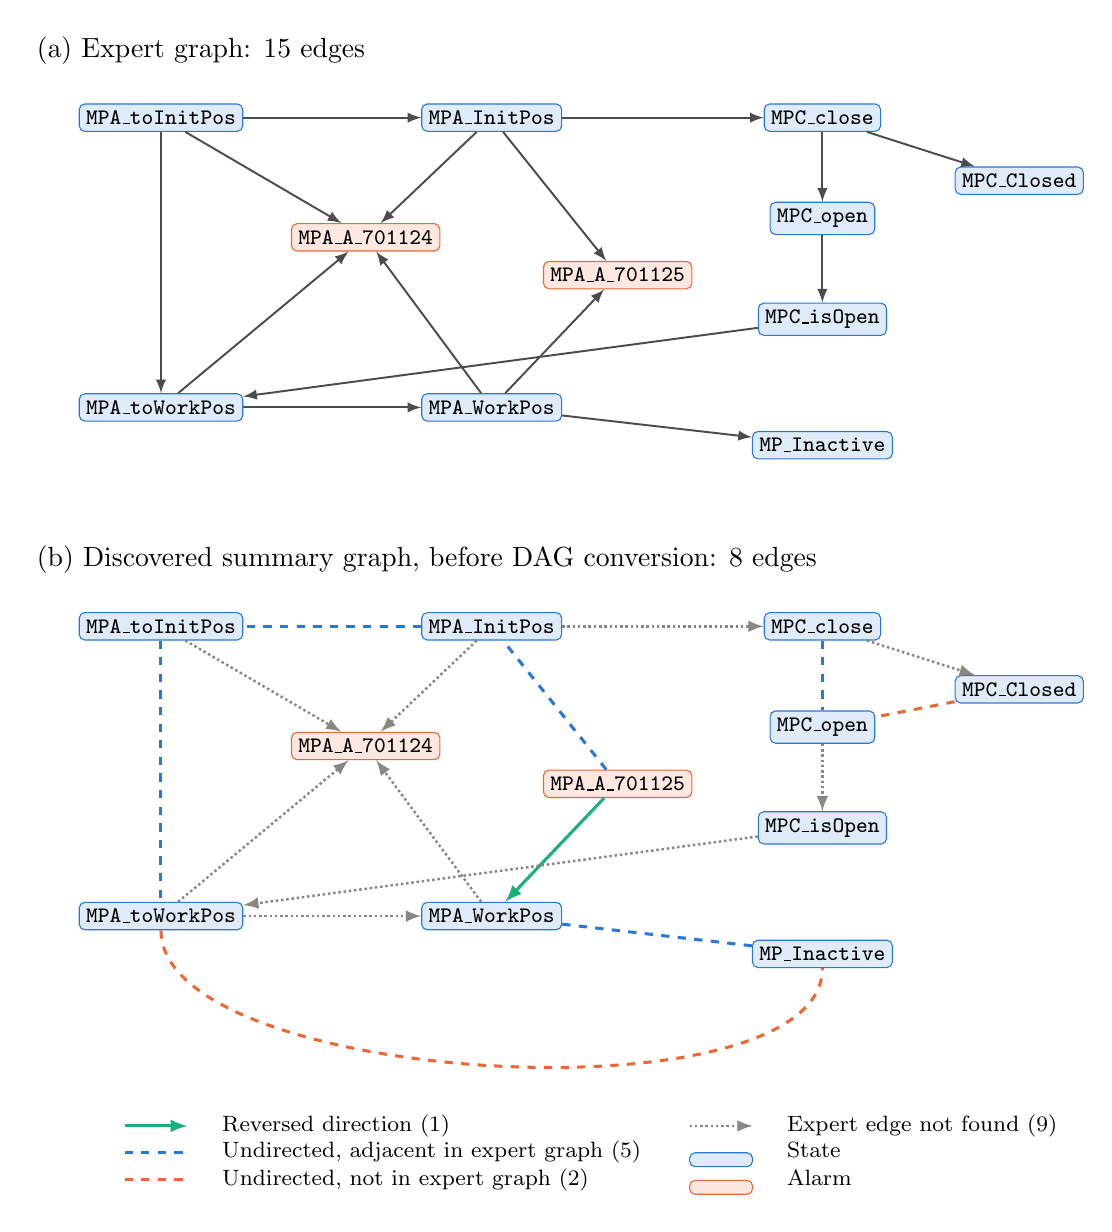
\begin{tikzpicture}[>=latex,
  st/.style={draw=figblue, fill=figblue!15, rounded corners=2pt, inner sep=2.5pt, font=\footnotesize\ttfamily},
  al/.style={draw=figorange, fill=figorange!15, rounded corners=2pt, inner sep=2.5pt, font=\footnotesize\ttfamily}]
\node[anchor=south west, font=\normalsize] at (-1.7, 0.55) {(a) Expert graph: 15 edges};
\node[st] (a-MPA-toInitPos) at (0, 0.00) {MPA\_toInitPos};
\node[st] (a-MPA-InitPos) at (4.2, 0.00) {MPA\_InitPos};
\node[st] (a-MPC-close) at (8.4, 0.00) {MPC\_close};
\node[st] (a-MPC-Closed) at (10.9, -0.80) {MPC\_Closed};
\node[st] (a-MPC-open) at (8.4, -1.28) {MPC\_open};
\node[st] (a-MPC-isOpen) at (8.4, -2.56) {MPC\_isOpen};
\node[al] (a-MPA-A-701124) at (2.6, -1.52) {MPA\_A\_701124};
\node[al] (a-MPA-A-701125) at (5.8, -2.00) {MPA\_A\_701125};
\node[st] (a-MPA-toWorkPos) at (0, -3.68) {MPA\_toWorkPos};
\node[st] (a-MPA-WorkPos) at (4.2, -3.68) {MPA\_WorkPos};
\node[st] (a-MP-Inactive) at (8.4, -4.16) {MP\_Inactive};
\draw[->, draw=black!70, line width=0.7pt] (a-MPA-InitPos) -- (a-MPA-A-701124);
\draw[->, draw=black!70, line width=0.7pt] (a-MPA-InitPos) -- (a-MPA-A-701125);
\draw[->, draw=black!70, line width=0.7pt] (a-MPA-InitPos) -- (a-MPC-close);
\draw[->, draw=black!70, line width=0.7pt] (a-MPA-toInitPos) -- (a-MPA-A-701124);
\draw[->, draw=black!70, line width=0.7pt] (a-MPA-toInitPos) -- (a-MPA-InitPos);
\draw[->, draw=black!70, line width=0.7pt] (a-MPA-toInitPos) -- (a-MPA-toWorkPos);
\draw[->, draw=black!70, line width=0.7pt] (a-MPA-toWorkPos) -- (a-MPA-A-701124);
\draw[->, draw=black!70, line width=0.7pt] (a-MPA-toWorkPos) -- (a-MPA-WorkPos);
\draw[->, draw=black!70, line width=0.7pt] (a-MPA-WorkPos) -- (a-MP-Inactive);
\draw[->, draw=black!70, line width=0.7pt] (a-MPA-WorkPos) -- (a-MPA-A-701124);
\draw[->, draw=black!70, line width=0.7pt] (a-MPA-WorkPos) -- (a-MPA-A-701125);
\draw[->, draw=black!70, line width=0.7pt] (a-MPC-close) -- (a-MPC-Closed);
\draw[->, draw=black!70, line width=0.7pt] (a-MPC-close) -- (a-MPC-open);
\draw[->, draw=black!70, line width=0.7pt] (a-MPC-isOpen) -- (a-MPA-toWorkPos);
\draw[->, draw=black!70, line width=0.7pt] (a-MPC-open) -- (a-MPC-isOpen);
\node[anchor=south west, font=\normalsize] at (-1.7, -5.91) {(b) Discovered summary graph, before DAG conversion: 8 edges};
\node[st] (b-MPA-toInitPos) at (0, -6.46) {MPA\_toInitPos};
\node[st] (b-MPA-InitPos) at (4.2, -6.46) {MPA\_InitPos};
\node[st] (b-MPC-close) at (8.4, -6.46) {MPC\_close};
\node[st] (b-MPC-Closed) at (10.9, -7.26) {MPC\_Closed};
\node[st] (b-MPC-open) at (8.4, -7.74) {MPC\_open};
\node[st] (b-MPC-isOpen) at (8.4, -9.02) {MPC\_isOpen};
\node[al] (b-MPA-A-701124) at (2.6, -7.98) {MPA\_A\_701124};
\node[al] (b-MPA-A-701125) at (5.8, -8.46) {MPA\_A\_701125};
\node[st] (b-MPA-toWorkPos) at (0, -10.14) {MPA\_toWorkPos};
\node[st] (b-MPA-WorkPos) at (4.2, -10.14) {MPA\_WorkPos};
\node[st] (b-MP-Inactive) at (8.4, -10.62) {MP\_Inactive};
\draw[draw=figblue, line width=1.1pt, dashed] (b-MPA-A-701125) -- (b-MPA-InitPos);
\draw[->, draw=figgreen, line width=1.1pt] (b-MPA-A-701125) -- (b-MPA-WorkPos);
\draw[draw=figblue, line width=1.1pt, dashed] (b-MPA-InitPos) -- (b-MPA-toInitPos);
\draw[draw=figblue, line width=1.1pt, dashed] (b-MPA-WorkPos) -- (b-MP-Inactive);
\draw[draw=figblue, line width=1.1pt, dashed] (b-MPA-toInitPos) -- (b-MPA-toWorkPos);
\draw[draw=figorange, line width=1.1pt, dashed] (b-MPA-toWorkPos.south) to[out=-90, in=-90, looseness=0.6] (b-MP-Inactive.south);
\draw[draw=figorange, line width=1.1pt, dashed] (b-MPC-Closed) -- (b-MPC-open);
\draw[draw=figblue, line width=1.1pt, dashed] (b-MPC-close) -- (b-MPC-open);
\draw[->, draw=figgrey, line width=0.9pt, densely dotted] (b-MPA-InitPos) -- (b-MPA-A-701124);
\draw[->, draw=figgrey, line width=0.9pt, densely dotted] (b-MPA-InitPos) -- (b-MPC-close);
\draw[->, draw=figgrey, line width=0.9pt, densely dotted] (b-MPA-toInitPos) -- (b-MPA-A-701124);
\draw[->, draw=figgrey, line width=0.9pt, densely dotted] (b-MPA-toWorkPos) -- (b-MPA-A-701124);
\draw[->, draw=figgrey, line width=0.9pt, densely dotted] (b-MPA-toWorkPos) -- (b-MPA-WorkPos);
\draw[->, draw=figgrey, line width=0.9pt, densely dotted] (b-MPA-WorkPos) -- (b-MPA-A-701124);
\draw[->, draw=figgrey, line width=0.9pt, densely dotted] (b-MPC-close) -- (b-MPC-Closed);
\draw[->, draw=figgrey, line width=0.9pt, densely dotted] (b-MPC-isOpen) -- (b-MPA-toWorkPos);
\draw[->, draw=figgrey, line width=0.9pt, densely dotted] (b-MPC-open) -- (b-MPC-isOpen);
\node[anchor=north, font=\footnotesize] at (5.45, -12.52) {\begin{tabular}{@{}cl@{\hspace{6mm}}cl@{}}
\tikz[baseline=-0.6ex]\draw[->, draw=figgreen, line width=1.1pt] (0,0) -- (0.8,0); & Reversed direction (1) & \tikz[baseline=-0.6ex]\draw[->, draw=figgrey, line width=0.9pt, densely dotted] (0,0) -- (0.8,0); & Expert edge not found (9) \\
\tikz[baseline=-0.6ex]\draw[draw=figblue, line width=1.1pt, dashed] (0,0) -- (0.8,0); & Undirected, adjacent in expert graph (5) & \tikz[baseline=-0.6ex]\node[st, minimum width=8mm] {};& State \\
\tikz[baseline=-0.6ex]\draw[draw=figorange, line width=1.1pt, dashed] (0,0) -- (0.8,0); & Undirected, not in expert graph (2) & \tikz[baseline=-0.6ex]\node[al, minimum width=8mm] {};& Alarm \\
\end{tabular}};
\end{tikzpicture}
